\documentclass[tikz,border=9pt]{standalone}
\usepackage[T1]{fontenc}
\usepackage{lmodern,amsmath}
\usetikzlibrary{arrows.meta}
\definecolor{ink}{HTML}{183444}
\definecolor{blue}{HTML}{1B6780}
\definecolor{amber}{HTML}{B56722}
\begin{document}
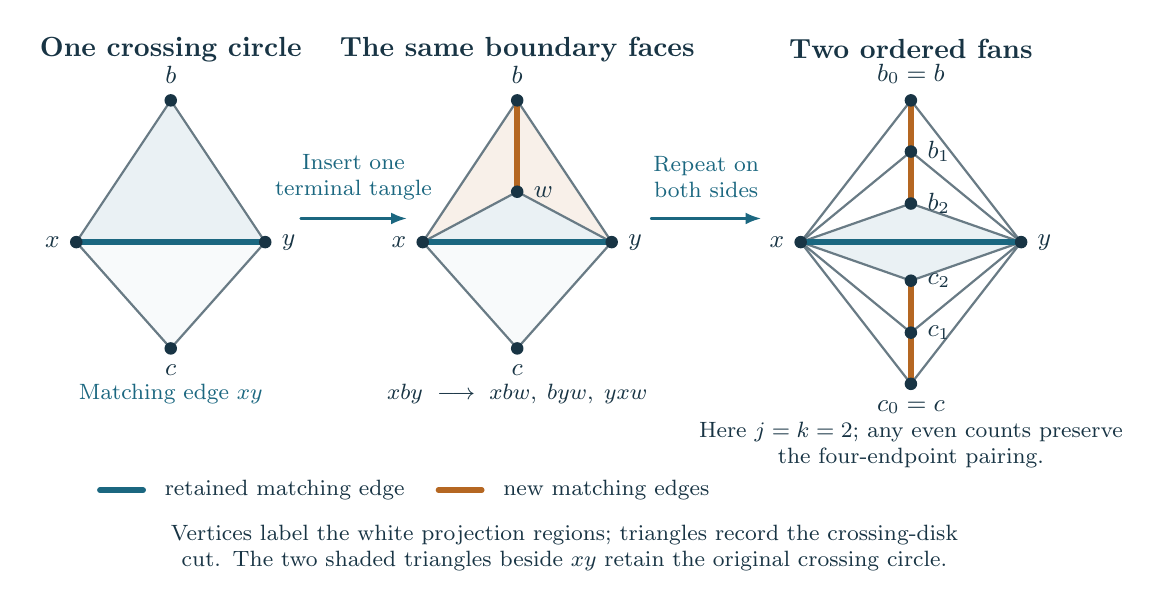
\begin{tikzpicture}[x=1cm,y=1cm,font=\small,text=ink,
 line cap=round,line join=round,
 edge/.style={draw=ink!65,line width=.8pt},
 old/.style={draw=blue,line width=2pt},
 fresh/.style={draw=amber,line width=2pt},
 dot/.style={circle,fill=ink,inner sep=1.6pt},
 move/.style={-{Latex[length=2mm]},draw=blue,line width=.9pt}]
% These are the white-face triangulations, with the inherited matching.
\begin{scope}[shift={(-5.0,0)}]
 \coordinate (x) at (-1.2,0); \coordinate (y) at (1.2,0);
 \coordinate (b) at (0,1.8); \coordinate (c) at (0,-1.35);
 \fill[blue!9] (x)--(b)--(y)--cycle;
 \fill[blue!3] (x)--(c)--(y)--cycle;
 \draw[edge] (x)--(b)--(y)--(c)--cycle;
 \draw[old] (x)--(y);
 \foreach \p/\pos in {x/left,y/right,b/above,c/below}{
   \node[dot,label=\pos:{$\p$}] at (\p) {};
 }
 \node[font=\bfseries] at (0,2.45) {One crossing circle};
 \node[text=blue,font=\footnotesize] at (0,-1.93) {Matching edge $xy$};
\end{scope}
\draw[move] (-3.35,.3)--(-2.0,.3);
\node[align=center,font=\footnotesize,text=blue] at (-2.68,.83)
 {Insert one\\terminal tangle};
\begin{scope}[shift={(-.6,0)}]
 \coordinate (x) at (-1.2,0); \coordinate (y) at (1.2,0);
 \coordinate (b) at (0,1.8); \coordinate (c) at (0,-1.35);
 \coordinate (w) at (0,.64);
 \fill[amber!10] (x)--(b)--(w)--cycle;
 \fill[amber!10] (b)--(y)--(w)--cycle;
 \fill[blue!9] (x)--(w)--(y)--cycle;
 \fill[blue!3] (x)--(c)--(y)--cycle;
 \draw[edge] (x)--(b)--(y)--(c)--cycle;
 \draw[edge] (x)--(w)--(y);
 \draw[old] (x)--(y); \draw[fresh] (b)--(w);
 \foreach \p/\pos in {x/left,y/right,b/above,c/below}{
   \node[dot,label=\pos:{$\p$}] at (\p) {};
 }
 \node[dot,label=right:{$w$}] at (w) {};
 \node[font=\bfseries] at (0,2.45) {The same boundary faces};
 \node[font=\footnotesize,align=center] at (0,-1.93)
  {$xby\ \longrightarrow\ xbw,\;byw,\;yxw$};
\end{scope}
\draw[move] (1.1,.3)--(2.5,.3);
\node[align=center,font=\footnotesize,text=blue] at (1.8,.83)
 {Repeat on\\both sides};
\begin{scope}[shift={(4.4,0)}]
 \coordinate (x) at (-1.4,0); \coordinate (y) at (1.4,0);
 \coordinate (b0) at (0,1.8); \coordinate (b1) at (0,1.15);
 \coordinate (b2) at (0,.49); \coordinate (c0) at (0,-1.8);
 \coordinate (c1) at (0,-1.15); \coordinate (c2) at (0,-.49);
 \fill[blue!9] (x)--(b2)--(y)--(c2)--cycle;
 \foreach \p in {b0,b1,b2,c0,c1,c2}{\draw[edge] (x)--(\p)--(y);}
 \draw[old] (x)--(y);
 \draw[fresh] (b0)--(b1)--(b2); \draw[fresh] (c0)--(c1)--(c2);
 \node[dot,label=left:{$x$}] at (x) {};
 \node[dot,label=right:{$y$}] at (y) {};
 \node[dot,label=above:{$b_0=b$}] at (b0) {};
 \node[dot,label=right:{$b_1$}] at (b1) {};
 \node[dot,label=right:{$b_2$}] at (b2) {};
 \node[dot,label=below:{$c_0=c$}] at (c0) {};
 \node[dot,label=right:{$c_1$}] at (c1) {};
 \node[dot,label=right:{$c_2$}] at (c2) {};
 \node[font=\bfseries] at (0,2.45) {Two ordered fans};
 \node[font=\footnotesize,align=center] at (0,-2.58)
  {Here $j=k=2$; any even counts preserve\\the four-endpoint pairing.};
\end{scope}
\draw[old] (-5.9,-3.15)--(-5.35,-3.15);
\node[anchor=west,font=\footnotesize] at (-5.2,-3.15) {retained matching edge};
\draw[fresh] (-1.6,-3.15)--(-1.05,-3.15);
\node[anchor=west,font=\footnotesize] at (-.9,-3.15) {new matching edges};
\node[align=center,font=\footnotesize,text width=13.4cm] at (0,-3.88)
 {Vertices label the white projection regions; triangles record the crossing-disk cut.
  The two shaded triangles beside $xy$ retain the original crossing circle.};
\end{tikzpicture}
\end{document}
